%%%%%%%%%%%%%%%%%%%%%%%%%%%%%%%%%%%%%%%%%%%%%%%%%%%%%%%%%%%%%%%
%
% Welcome to Overleaf --- just edit your LaTeX on the left,
% and we'll compile it for you on the right. If you open the
% 'Share' menu, you can invite other users to edit at the same
% time. See www.overleaf.com/learn for more info. Enjoy!
%
%%%%%%%%%%%%%%%%%%%%%%%%%%%%%%%%%%%%%%%%%%%%%%%%%%%%%%%%%%%%%%%


% Inbuilt themes in beamer
\documentclass{beamer}

% Theme choice:
\usetheme{CambridgeUS}

% Title page details: 
\title{Assignment 6}% \\ Indian Institute of Technology Hyderabad} 
\author{Pradeep Mundlik \\ AI21BTECH11022}
\date{\today}
% \logo{\large \LaTeX{}}


\begin{document}

% Title page frame
\begin{frame}
    \titlepage 
\end{frame}

% Remove logo from the next slides
% \logo{}


% Outline frame
\begin{frame}{Outline}
    \tableofcontents
\end{frame}


% Lists frame
\section{Question}
\begin{frame}{Question}
    Let X denote the number of hours you study during a randomly selected
    school day. The probability that X can take values x, has the following form, where
    k is some unknown constant. \\
    \begin{align}
        Pr(X = x) = 
        \begin{cases}
            0.1 & x = 0 \\
            kx & x = 1,2 \\
            k\left(5-x\right) & x = 3,4 \\
            0 & otherwise
        \end{cases}
    \end{align}
    (i) Find the value of k.\\
    (ii) What is the probability that you study at least two hours? Exactly two hours?
    Atmost two hours? 
\end{frame}

\section{Answer}
\begin{frame}{Answer}
    X is Random variable which can take following values with respective probabilities. 
    \begin{table}[htb]
        \tiny
        %\begin{center}
        \resizebox{\columnwidth}{!}{
        \begin{tabular}{|c|c|c|c|c|c|}
        \hline
        % \begin{tabularx}{\linewidth} {lX}
         X & 0 & 1 & 2 & 3 & 4 \\ 
         \hline
         P(X) & 0.1 & k & 2k & 2k & k\\  
         \hline
        %  \end{tabularx}
        \end{tabular}
        }
        \caption{}
        \end{table}
    \end{frame}
    
    \subsection{Part(i)}
    \begin{frame}{Part(i) -}
        
        We know that
        \begin{align}
            \sum_{i = 1}^{n} p_i  = 1
        \end{align}
        Therefore
        \begin{align}
            \implies &0.1 + k + 2k + 2k + k = 1 \\
            \implies &0.1 + 6k = 1 \\
            \implies &6k = 0.90 \\
            \implies &k = \left(\frac{0.90}{6}\right) \\
            \implies &k = 0.15
        \end{align}
    \end{frame}
    \begin{frame}
        Now, probabilities become, 
        \begin{table}[htb]
            \tiny
            %\begin{center}
            \resizebox{\columnwidth}{!}{
            \begin{tabular}{|c|c|c|c|c|c|}
            \hline
            % \begin{tabularx}{\linewidth} {lX}
             X & 0 & 1 & 2 & 3 & 4 \\ 
             \hline
             P(X) & 0.1 & 0.15 & 0.30 & 0.30 & 0.15\\  
             \hline
            %  \end{tabularx}
            \end{tabular}
            }
            \caption{}
            \end{table}
\end{frame}

\begin{frame}
    \begin{figure}[!ht]
        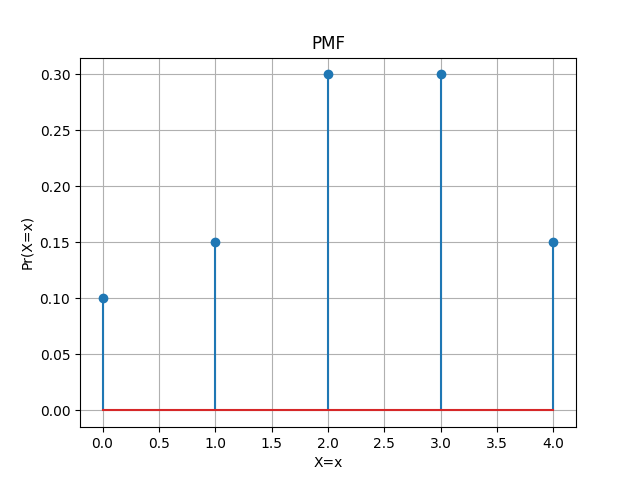
\includegraphics[width=4in, height=3in]{figures/pmf.png}
        \caption{Probability Mass Function.}
    \end{figure}
\end{frame}

\begin{frame}
    \begin{figure}[!ht]
        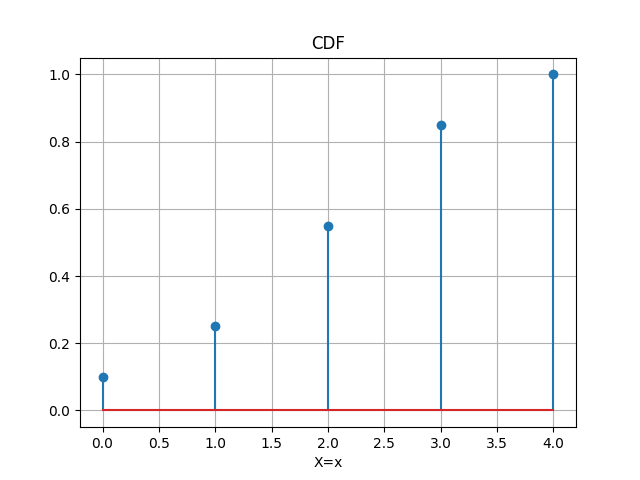
\includegraphics[width=4in, height=3in]{figures/cdf.png}
        \caption{Cumulative Distribution Function.}
    \end{figure}
\end{frame}

\subsection{Part(ii)}
    \begin{itemize}
    \begin{frame}{Part(ii) - }
        \item 
        Let A is an event \\
        A: You atleast study two hours \\
        So, 
        \begin{align}
            Pr(A)  &= Pr(X\geq 2) \\
            &= Pr(X=2) + Pr(X=3) + Pr(X=4) \\
            &= 2k + 2k + k \\
            &= 5k \\
            &= 5\times 0.15 \\
            &= 0.75
        \end{align}
        Hence, probability of you study atleast two hours is 0.75. \\
    \end{frame}
    \begin{frame}
        \item 
        Let B is an event \\
        B: You study exactly two hours \\
        So, 
        \begin{align}
            Pr(B)  &= Pr(X=2) \\
            &= 2k \\
            &= 2\times 0.15 \\
            &= 0.30
        \end{align}
        Hence, probability of you study exactly two hours is 0.30. \\
    \end{frame}
    \begin{frame}
        \item 
        Let C is an event \\
        C: You study atmost two hours \\
        So, 
        \begin{align}
            Pr(C)  &= Pr(X\leq 2) \\
            &= Pr(X=0) + Pr(X=1) + Pr(X=2) \\
            &= 0.1 + k + 2k \\
            &= 0.1 + 3k \\
            &= 0.1 + 3\times 0.15 \\
            &= 0.1 + 0.45 \\
            &= 0.55
        \end{align}
        Hence, probability of you study atmost two hours is 0.55. \\
    \end{frame}
\end{itemize}
\end{document}